\documentclass[11pt,a4paper,bibliography=totocnumbered]{scrartcl}
\usepackage[utf8]{inputenc}
\usepackage[british]{babel}
%\usepackage{amsmath}
%\usepackage{amsfonts}
%\usepackage{amssymb}
\usepackage[footsepline]{scrlayer-scrpage}
\usepackage{tabu}
\usepackage{placeins}
%\usepackage{longtable}
\usepackage{multirow}
\usepackage{setspace}
%\usepackage{graphicx}
%\usepackage{pgfplots}
\usepackage{hyperref}
\usepackage{url}
\usepackage{titling}
\usepackage[backend=biber,sorting=none]{biblatex}
\usepackage{csquotes}
\usepackage{pdfpages}
\usepackage{epstopdf}
\usepackage{graphicx}
\usepackage{subfig}
\usepackage{array}
%\usepackage{enumitem}
\usepackage[backgroundcolor=lightgray]{todonotes}

%\pgfplotsset{width=12cm,height=6cm,compat=1.11}

% Constants
\def\mytitle{Tomcat Native 2}
\def\myauthor{Jocelyn Thode and Simon Brulhart}
\def\theclient{Red Hat}

\pagestyle{scrheadings}

\ihead{\mytitle}
\chead{}
\cfoot{}
\ifoot{Initial plan}
\ofoot{\thepage}

\posttitle{\end{center}\begin{center}\LARGE Final Report\end{center}}

\author{\myauthor\\ \href{mailto:jocelyn.thode@unifr.ch}{jocelyn.thode@unifr.ch} \\ \href{mailto:simon.brulhart@unifr.ch}{simon.brulhart@unifr.ch}}
\title{\huge \textbf{\mytitle}}

\bibliography{final_report}

\begin{document}

\graphicspath{{figures/}}

\begin{titlingpage}

\maketitle

\begin{abstract}
\mytitle{} is a project mandated by Red Hat. It aims at providing a JNI wrapper for OpenSSL for use in both Undertow and Tomcat. This project is the practical part of the R\&D Workshop course given at the University of Neuchâtel as part of the Joint Master in Computer Science.
\end{abstract}

\begin{figure}[b]
\centering
\subfloat{
\includegraphics[height=1.8cm]{unine.eps}}
\qquad
\subfloat{
\includegraphics[height=1.5cm]{jmcs.png}}
\qquad
\subfloat{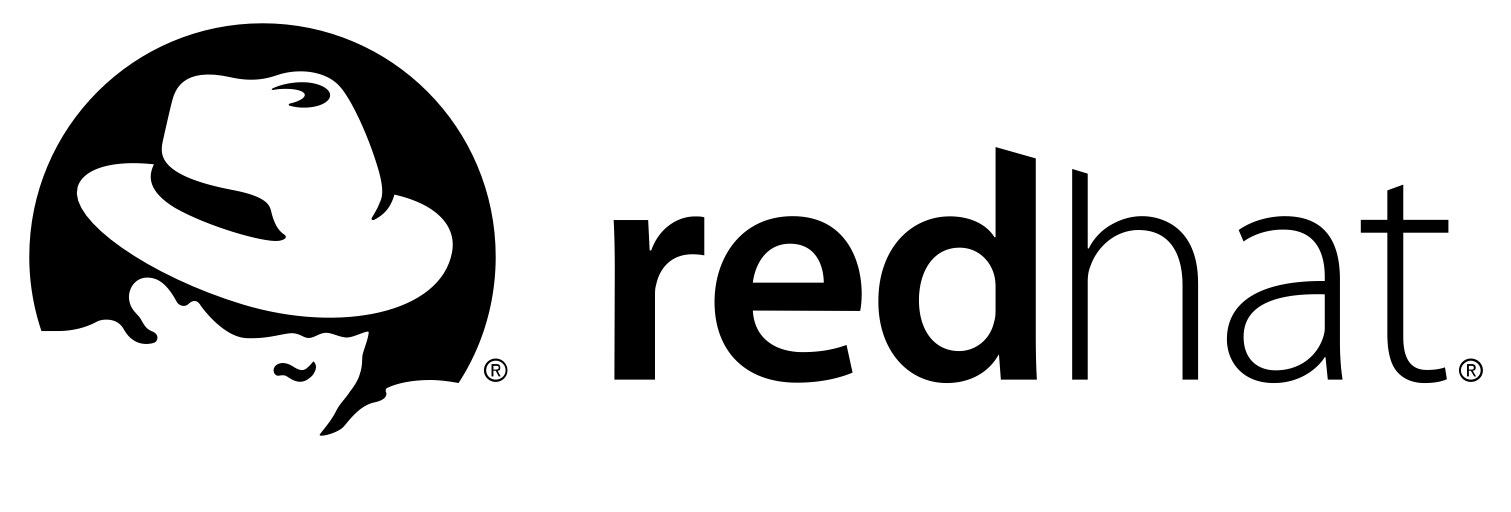
\includegraphics[height=1.6cm]{redhat-logo.png}}
\end{figure}

\end{titlingpage}

\pagebreak

\setcounter{tocdepth}{2}
\tableofcontents
\listoffigures

\pagebreak

\section{Project description}

\subsection{Project context}
For this project we are working with \theclient{} which is a multinational software company that provides open-source software and technical support to enterprises\autocite{redhat}.
At the moment, Tomcat\autocite{tomcat} and Undertow\autocite{undertow} are among the most used Java web servers. Both rely on TLS/SSL to encrypt and secure communications between a client and a server. To achieve good performance Tomcat Native\autocite{tomcat-native} provides access to OpenSSL in Tomcat. It uses Apache Portable Runtime (APR) to do so. 
Unfortunately, Undertow isn't compatible with Tomcat Native at the moment.
Until last year, the APR would manage the encrypted sockets by itself. However this implied a lot of C code to maintain. To ease maintenance, some work has been done to use OpenSSL APIs directly instead. This works well enough despite some acceptable performance penalty. However the APR still provides the bindings to these APIs.
We now want to strip the current solution of the APR and make the result compatible with Undertow.

Figure \ref{fig:current} shows an overview of the different ways to use TLS/SSL in Tomcat. This figure describes the path taken by a piece of data, going from Tomcat/Undertow to the OS network layer. There is a different color for each way to use TLS/SSL.

\subsection{Goals and objectives of the project}

Our project aims to refactor Tomcat Native to drop APR and only rely on our own JNI wrapper to interface with OpenSSL. This should make Tomcat Native much more maintainable while keeping great performance when using TLS/SSL. The project also aims to make the resulting \mytitle{} usable in Undertow while keeping the compatibility with Tomcat.
This means we need to :
\begin{enumerate}
\item Study the source code of Tomcat Native, Undertow and some experiments already done to use OpenSSL in Undertow.
\item Remove all APR code present in Tomcat Native
\item Abstract Tomcat Native to be used in Tomcat and Undertow
\item Provide good documentation so that the open-source community can use the project
\item Run benchmarks to test the implementation on multiple platforms
\item Extend the OpenSSL support by adding JNIs for more features
\end{enumerate}

Figure \ref{fig:goal} shows what is expected at the end of the project.

\section{Project organization}
\label{sec:org}

This project requires us to read some documentation and source code. We also need to write reports and presentations. To keep the code base clean, we decided to adopt the same strategy as Numa de Montmollin last year and split our work in two different repositories on Github.

\href{https://github.com/jocelynthode/tomcat-native2-doc}{tomcat-native2-doc} is the repository documenting the progress of our project. We put every report and presentation in the repo. This repo also contains a wiki which hosts the logbook, work plan and our different articles. The articles are useful to share our findings and more importantly to not forget about them.

\href{https://github.com/jocelynthode/tomcat-native2}{tomcat-native2} is the repository dedicated to the code. This repo includes our implementation, and the documentation directly concerning it. For example, it should contain a ReadMe describing the building process and the main purpose of the project.

\section{Results \& Realization}
\todo[inline] {realization and results, short explanation of the deliverables}

\section{Recommendations}
\todo[inline] {recommendations, project limitations, outstanding issues,future work}

\newpage
\printbibliography

\begin{figure}[!h]
\begin{center}
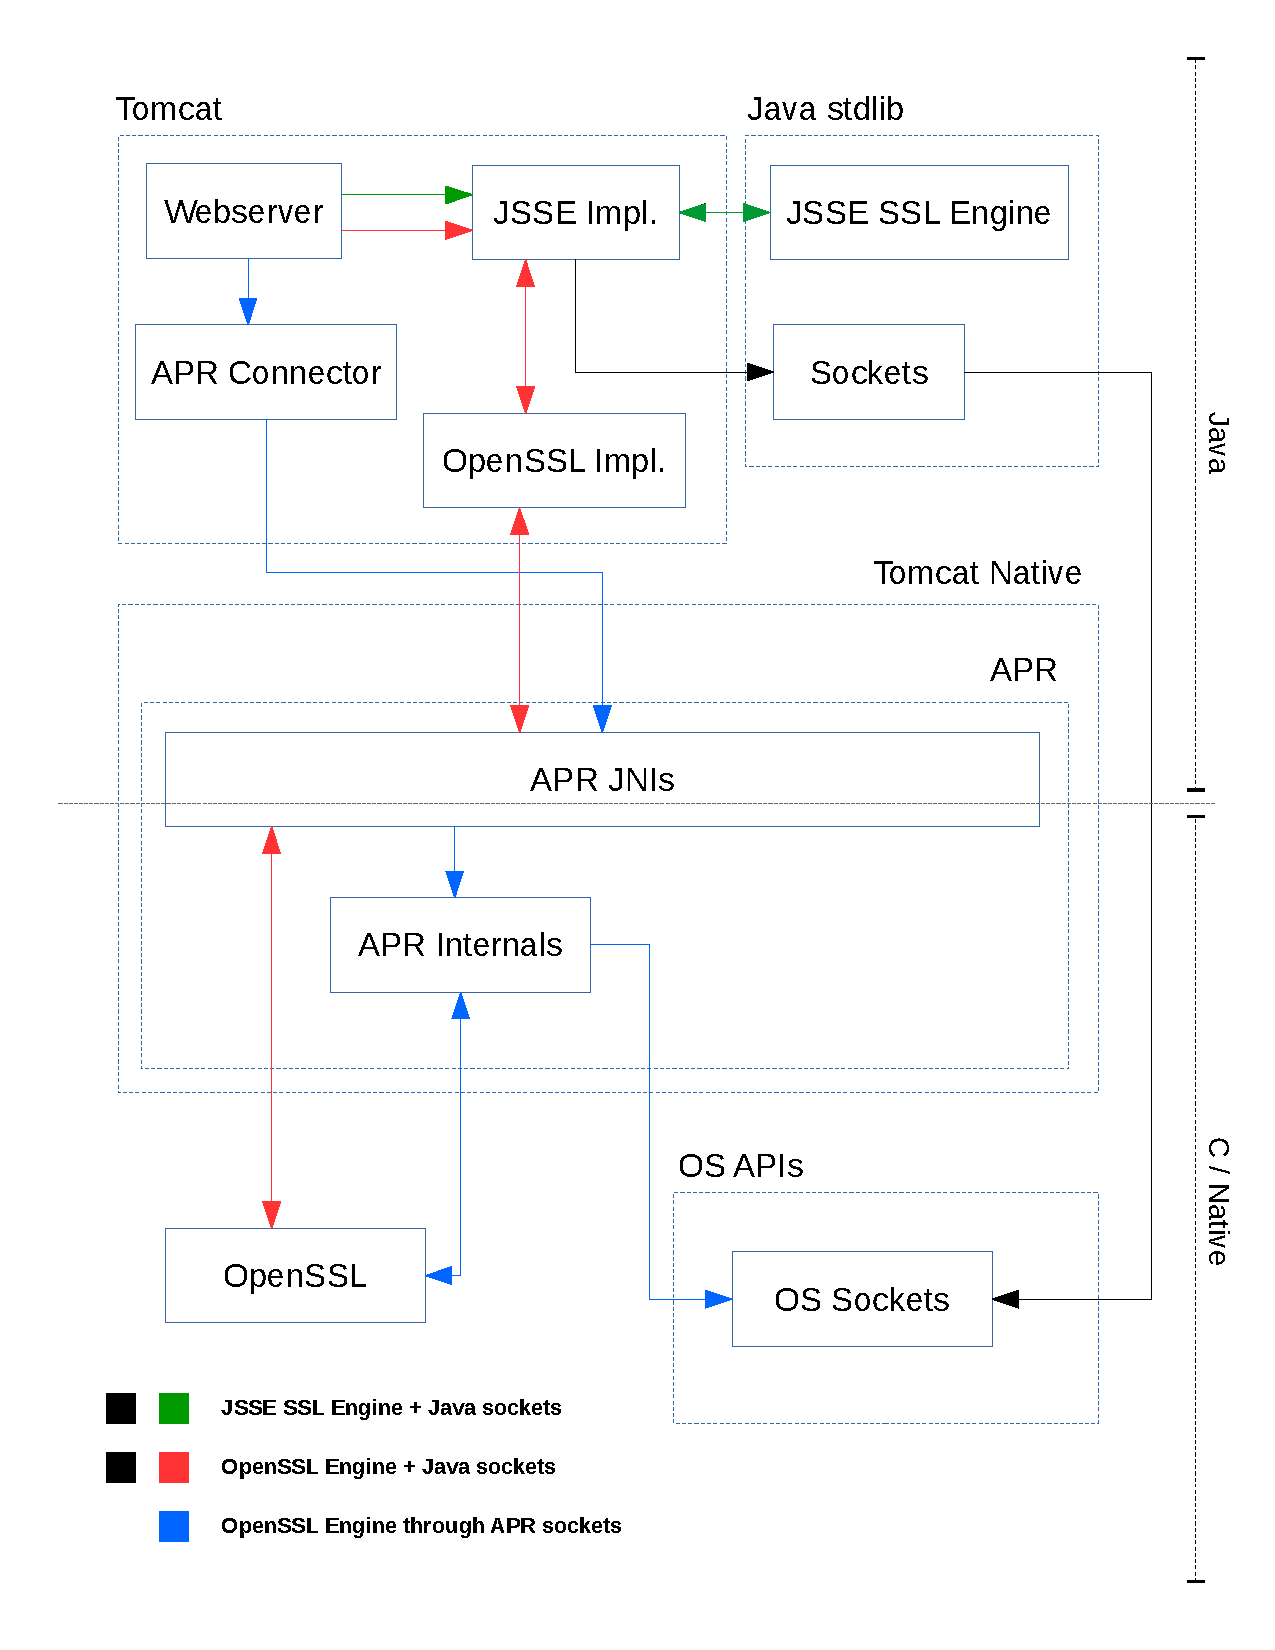
\includegraphics[scale=0.7]{diagram_current_way.pdf}
\end{center}
\caption{\textbf{Diagram showing the different ways to use TLS/SSL in Tomcat.}}
\label{fig:current}
\end{figure}

\begin{figure}[!h]
\begin{center}
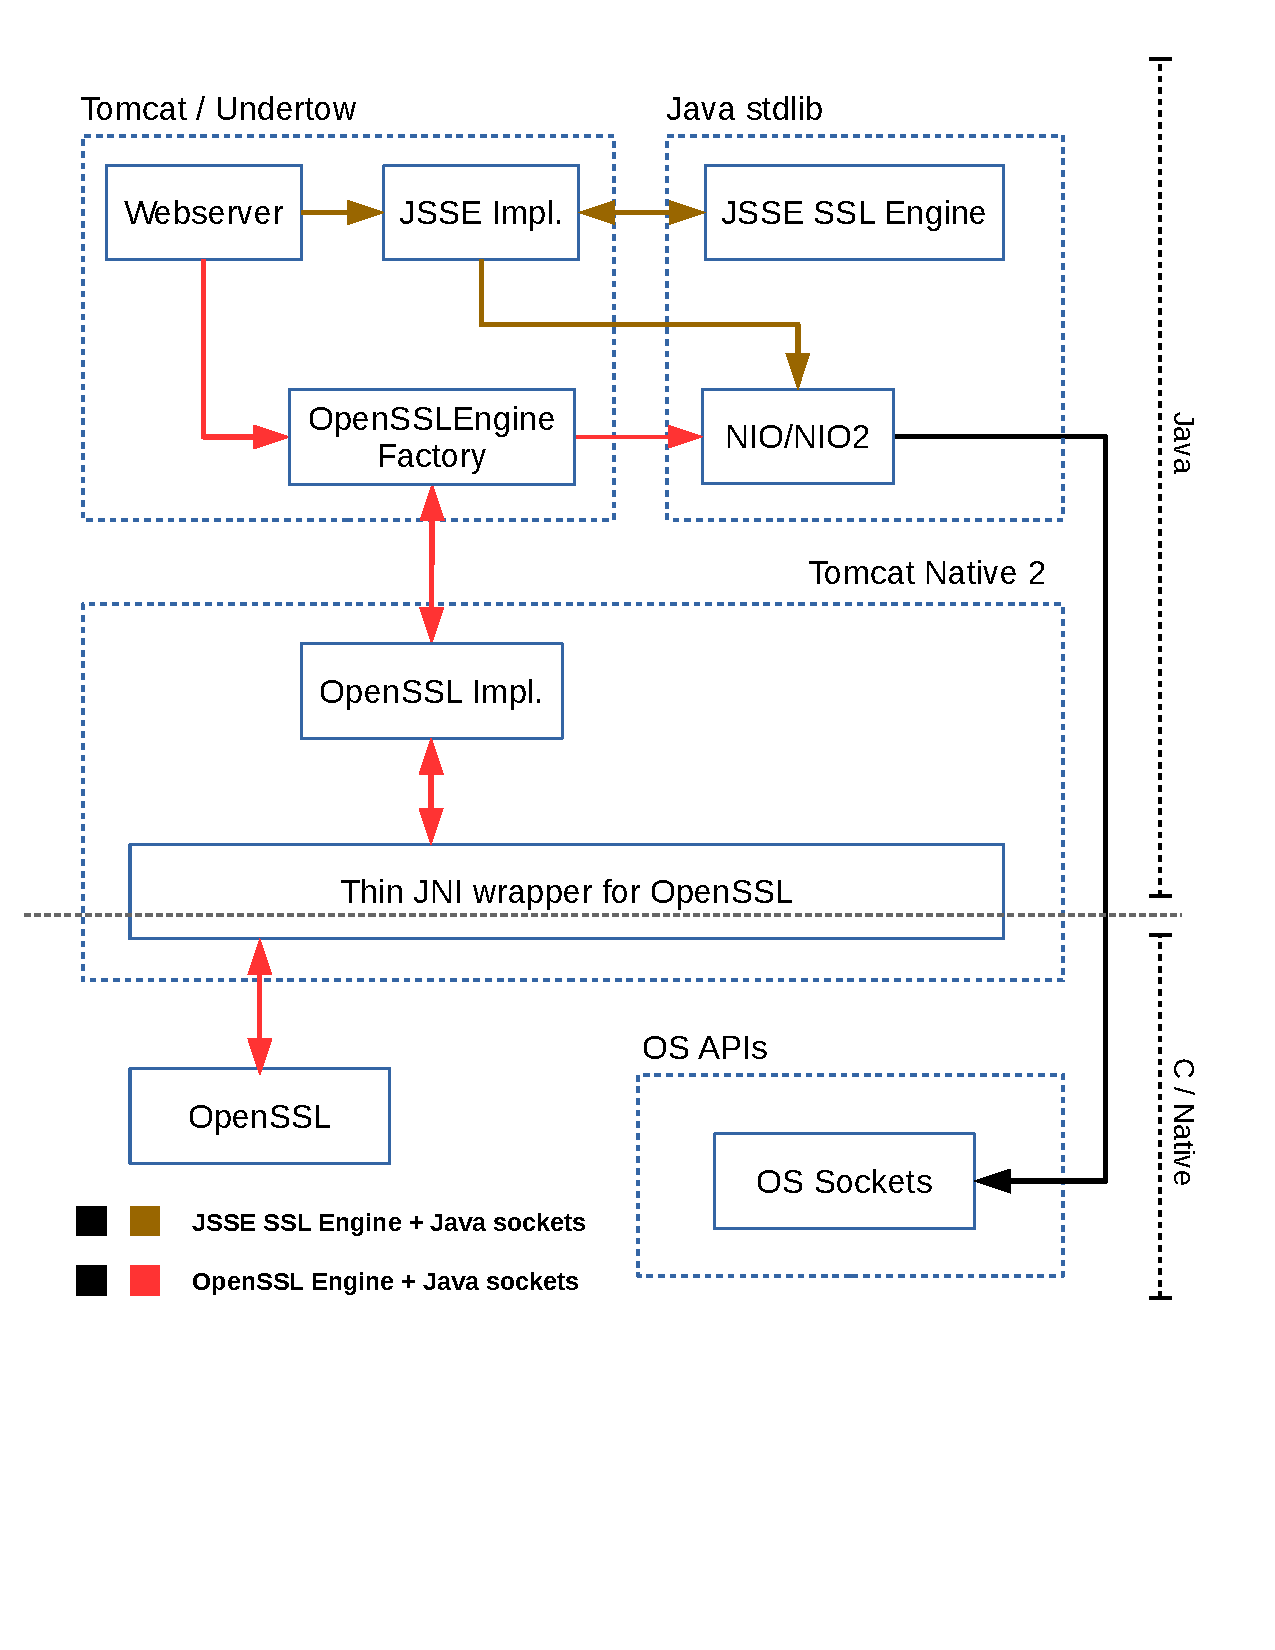
\includegraphics[scale=0.7]{diagram_goal.pdf}
\end{center}
\caption{\textbf{Diagram showing the expected end result of our project.}}
\label{fig:goal}
\end{figure}

\FloatBarrier

\end{document}